\documentclass[11pt]{report}

\usepackage[margin=1.1in]{geometry}
\usepackage[T1]{fontenc}
\usepackage{lmodern}
\usepackage{amsmath,amssymb,bm,mathtools}
\usepackage{graphicx}
\usepackage{xcolor}
\usepackage[colorlinks=true,linkcolor=blue!50!black,citecolor=blue!50!black,urlcolor=blue!50!black]{hyperref}

\setcounter{secnumdepth}{3}
\setcounter{tocdepth}{2}

% Summary box at the start of each lecture (plain LaTeX, no extra packages)
\newsavebox{\keyideasbox}
\newenvironment{keyideas}
    {\par\medskip\noindent\begin{lrbox}{\keyideasbox}%
     \begin{minipage}{\dimexpr\linewidth-2\fboxsep-2\fboxrule\relax}%
     \textbf{\sffamily Key ideas}\par\smallskip}
    {\end{minipage}\end{lrbox}%
     \fcolorbox{blue!35!black}{blue!3!white}{\usebox{\keyideasbox}}\par\medskip}

\title{\textbf{LLM-note}\\[4pt]
\large Lecture notes on the theory of neural networks}
\author{Lianghong Mo}
\date{}

\begin{document}

\maketitle
\tableofcontents

% ============================================================
% Lecture 1: overview of the three theoretical questions
% ============================================================
\chapter{Three Questions in Deep-Learning Theory}
\label{ch:lecture1}

\begin{keyideas}
\begin{itemize}
    \item A neural network is a parametrized family of functions; what it
    learns is fixed jointly by the architecture, the data, and the
    optimization algorithm.
    \item \textbf{Scaling:} which simple effective theory emerges as
    $N,n,L,W,C\to\infty$ (NTK, mean field, DMFT, Gaussian processes), and
    why these limits need not commute.
    \item \textbf{Feature learning:} a network learns the feature map
    $\Phi_\theta(x)$ itself, not only its coefficients; features are
    directions in activation space and can be stored in superposition.
    \item \textbf{Diffusion:} learning the score $\nabla_x\log\rho_t$ by
    denoising is enough to reverse a noising process and sample from
    $\rho_{\mathrm{data}}$.
\end{itemize}
\end{keyideas}

\section{Introduction}

A useful viewpoint is that a neural network is a \emph{parametrized family of functions}. 
We choose an architecture, which determines a family
\begin{equation}
    \left\{
    f_\theta:\mathcal X\rightarrow\mathcal Y
    \right\}_{\theta\in\Theta},
\end{equation}
and learning consists of selecting the parameter $\theta$ using data.

Thus there are three conceptually distinct ingredients:
\begin{enumerate}
    \item the \textbf{architecture}, which specifies the function class;
    \item the \textbf{data}, which provide information about the unknown target;
    \item the \textbf{optimization algorithm}, which determines which member of the
    function class is actually learned.
\end{enumerate}

One of the central questions in the theory of neural networks is therefore
\begin{equation}
    \boxed{
    \text{Architecture}
    +
    \text{Data}
    +
    \text{Optimization}
    \quad
    \Longrightarrow
    \quad
    \text{Learned function / representation}.
    }
\end{equation}


% ============================================================
\subsection{Definition of Neural Networks}

\subsubsection{Fully connected neural networks}

Consider an input
\begin{equation}
    x\in\mathbb R^{N_0}.
\end{equation}
Define
\begin{equation}
    z^{(0)}(x)=x.
\end{equation}
A fully connected neural network with $L+1$ layers is recursively defined by
\begin{equation}
    z^{(\ell+1)}(x)
    =
    W^{(\ell+1)}
    \phi\!\left(z^{(\ell)}(x)\right)
    +
    b^{(\ell+1)},
    \qquad
    \ell=0,\ldots,L,
\end{equation}
where
\begin{equation}
    W^{(\ell+1)}
    \in
    \mathbb R^{N_{\ell+1}\times N_\ell},
    \qquad
    b^{(\ell+1)}
    \in
    \mathbb R^{N_{\ell+1}},
\end{equation}
and $\phi$ is a nonlinear activation function applied componentwise.\footnote{With
this convention $\phi$ also acts on the raw input $z^{(0)}=x$. Lecture~2 uses
the equally common convention $z^{(1)}=W^{(1)}x+b^{(1)}$; nothing below
depends on the choice.}

Typical choices include
\begin{align}
    \mathrm{ReLU}(x)&=\max(0,x),\\
    \tanh(x)&=\frac{e^x-e^{-x}}{e^x+e^{-x}},\\
    \mathrm{GELU}(x)&=x\Phi(x),
\end{align}
where $\Phi$ is the standard Gaussian cumulative distribution function.

The output of the network is
\begin{equation}
    f_\theta(x)
    \equiv
    z^{(L+1)}(x),
\end{equation}
where the parameter set is
\begin{equation}
    \theta
    =
    \left\{
    W^{(1)},\ldots,W^{(L+1)},
    b^{(1)},\ldots,b^{(L+1)}
    \right\}.
\end{equation}

The nonlinear activation is essential. Without $\phi$, a composition of linear
layers would still be only a linear transformation:
\begin{equation}
    W^{(L)}W^{(L-1)}\cdots W^{(1)}x
    =
    W_{\mathrm{eff}}x.
\end{equation}


\subsubsection{Residual neural networks}

Instead of replacing the current representation at every layer, a residual
network learns a correction:
\begin{equation}
    z^{(\ell+1)}
    =
    z^{(\ell)}
    +
    F_{\theta_\ell}\!\left(z^{(\ell)}\right).
\end{equation}

A typical residual block is
\begin{equation}
    F_{\theta_\ell}(z)
    =
    W_2^{(\ell)}
    \phi\!\left(
        W_1^{(\ell)}z+b_1^{(\ell)}
    \right)
    +
    b_2^{(\ell)}.
\end{equation}

Therefore,
\begin{equation}
    z^{(\ell+1)}
    =
    z^{(\ell)}
    +
    W_2^{(\ell)}
    \phi\!\left(
        W_1^{(\ell)}z^{(\ell)}
        +
        b_1^{(\ell)}
    \right)
    +
    b_2^{(\ell)}.
\end{equation}

The important physical picture is that each layer makes only an incremental
update,
\begin{equation}
    \Delta z^{(\ell)}
    =
    F_{\theta_\ell}(z^{(\ell)}).
\end{equation}

In a formal continuum-depth limit, a residual network resembles a dynamical
system,
\begin{equation}
    \frac{dz(t)}{dt}
    =
    F_{\theta(t)}(z(t)),
\end{equation}
which motivates the connection between residual networks and differential
equations.


% ============================================================
\subsection{How Neural Networks Are Used}

Suppose there is an unknown target function
\begin{equation}
    f:\mathcal X\rightarrow\mathcal Y.
\end{equation}
We observe a training dataset
\begin{equation}
    \mathcal D
    =
    \left\{
    (x_i,y_i)
    \right\}_{i=1}^{n},
    \qquad
    y_i=f(x_i),
\end{equation}
where $n$ denotes the number of training samples.

The standard supervised-learning procedure is:

\begin{enumerate}
    \item \textbf{Data:}
    observe
    \begin{equation}
        \left\{
        (x_i,f(x_i))
        \right\}_{i=1}^n.
    \end{equation}
    The goal is to infer the unknown function $f$ from finitely many observations.

    \item \textbf{Initialization:}
    choose an initial parameter
    \begin{equation}
        \theta_0
        \sim
        P_{\mathrm{init}}.
    \end{equation}

    \item \textbf{Optimization:}
    minimize a loss function. For regression, a common choice is
    \begin{equation}
        \mathcal L(\theta)
        =
        \frac{1}{2n}
        \sum_{i=1}^n
        \left\|
        f(x_i)-f_\theta(x_i)
        \right\|^2.
    \end{equation}

    Gradient descent gives
    \begin{equation}
        \theta_{t+1}
        =
        \theta_t
        -
        \eta
        \nabla_\theta
        \mathcal L(\theta_t),
    \end{equation}
    where $\eta$ is the learning rate.

    In practice one usually uses stochastic gradient descent,
    \begin{equation}
        \theta_{t+1}
        =
        \theta_t
        -
        \eta
        \widehat{\nabla_\theta \mathcal L},
    \end{equation}
    where the gradient is estimated from a minibatch.

    \item \textbf{Generalization / test:}
    for a new point $x_{\mathrm{new}}$ that was not in the training set,
    ask whether
    \begin{equation}
        f(x_{\mathrm{new}})
        \approx
        f_{\theta_{\mathrm{learned}}}(x_{\mathrm{new}}).
    \end{equation}
\end{enumerate}

A neural network is therefore not useful merely because it can fit the training
data. The central problem is whether it can \emph{generalize}.


% ============================================================
\subsection{Three Main Topics}

We focus on three broad theoretical questions:

\begin{enumerate}
    \item \textbf{Scaling laws and large-network limits:}
    What happens as the model size, dataset size, and computational budget
    become very large?

    \item \textbf{Feature learning and representation learning:}
    What internal representations does the neural network learn, and why do
    these representations help generalization?

    \item \textbf{Generative models, especially diffusion models:}
    How can a neural network learn an entire high-dimensional probability
    distribution and generate new samples from it?
\end{enumerate}


% ============================================================
\section{Topic I: Scaling Laws and Large-Network Limits}

\subsection{Basic Questions}

Modern neural networks involve several potentially large parameters:
\begin{align}
    N &=
    \text{number of model parameters},\\
    n &=
    \text{number of training samples},\\
    L &=
    \text{depth},\\
    W &=
    \text{width},\\
    C &=
    \text{computational budget}.
\end{align}

The theoretical problem resembles statistical mechanics: instead of studying
one finite neural network in detail, we would like to identify simple laws that
emerge in appropriate large-scale limits.

Some central questions are:

\begin{enumerate}
    \item What happens when
    \begin{equation}
        N,n,L,W,C\rightarrow\infty?
    \end{equation}

    These limits need not commute. For example,
    \begin{equation}
        \lim_{n\rightarrow\infty}
        \lim_{W\rightarrow\infty}
    \end{equation}
    may describe a different regime from
    \begin{equation}
        \lim_{W\rightarrow\infty}
        \lim_{n\rightarrow\infty}.
    \end{equation}

    Therefore the interesting object is often a \emph{joint scaling limit},
    analogous to a thermodynamic limit.

    \item Does a complicated neural network reduce to a simpler effective theory
    in such a limit?

    \item Can performance at very large scale be predicted from experiments at
    relatively small scale?

    \item Which resource is the bottleneck:
    \begin{equation}
        \text{model size},\qquad
        \text{data},\qquad
        \text{optimization},\qquad
        \text{compute}?
    \end{equation}

    \item When does increasing the model size actually improve performance, and
    when does performance saturate?
\end{enumerate}


% ------------------------------------------------------------
\subsection{Empirical Scaling Laws}

Empirically, many machine-learning systems approximately obey power-law scaling
over a substantial range of scales.

For example, test loss may behave as
\begin{equation}
    \boxed{
    \mathcal L(C)
    =
    \mathcal L_\infty
    +
    A C^{-\beta},
    }
\end{equation}
where
\begin{equation}
    C=\text{compute},
\end{equation}
$\beta>0$ is a scaling exponent, and $\mathcal L_\infty$ is an irreducible
loss floor.

Similarly one may study
\begin{align}
    \mathcal L(N)
    &\approx
    \mathcal L_\infty
    +
    A_N N^{-\alpha_N},
    \\
    \mathcal L(n)
    &\approx
    \mathcal L_\infty
    +
    A_n n^{-\alpha_n}.
\end{align}

More generally,
\begin{equation}
    \mathcal L
    =
    \mathcal L(N,n,C,\ldots).
\end{equation}

The interesting theoretical questions are not only whether these power laws
exist, but also:
\begin{enumerate}
    \item why power laws emerge;
    \item whether the exponents are universal;
    \item how the exponents depend on the data distribution and architecture;
    \item how to optimally allocate a fixed computational budget between
    increasing $N$, increasing $n$, and training for longer.
\end{enumerate}


% ------------------------------------------------------------
\subsection{Optimization, Approximation, and Data Errors}

It is useful to conceptually decompose the total error into several pieces:
\begin{equation}
    \mathcal E_{\mathrm{total}}
    \sim
    \mathcal E_{\mathrm{approx}}
    +
    \mathcal E_{\mathrm{estimation}}
    +
    \mathcal E_{\mathrm{optimization}}.
\end{equation}

Here:
\begin{itemize}
    \item $\mathcal E_{\mathrm{approx}}$ measures whether the architecture is
    expressive enough to represent the desired function;

    \item $\mathcal E_{\mathrm{estimation}}$ arises because the training dataset
    is finite;

    \item $\mathcal E_{\mathrm{optimization}}$ measures whether the optimizer
    succeeds in finding a good parameter configuration.
\end{itemize}

Scaling the number of parameters only directly attacks the first of these.
Therefore increasing model size alone need not always improve performance.


% ------------------------------------------------------------
\subsection{Theoretical Approaches}

\subsubsection{Neural Tangent Kernel}

Consider the network output
\begin{equation}
    f_\theta(x).
\end{equation}
Linearize it around the initialization $\theta_0$:
\begin{equation}
    f_\theta(x)
    \approx
    f_{\theta_0}(x)
    +
    \nabla_\theta f_{\theta_0}(x)^T
    (\theta-\theta_0).
\end{equation}

Define the Neural Tangent Kernel
\begin{equation}
    K_{\mathrm{NTK}}(x,x')
    =
    \nabla_\theta f_{\theta_0}(x)^T
    \nabla_\theta f_{\theta_0}(x').
\end{equation}

In an appropriate infinite-width limit, the NTK becomes approximately
deterministic and changes very little during training.

The nonlinear neural-network training problem is then reduced to an effective
kernel regression problem.

The physical picture is
\begin{equation}
    \boxed{
    \text{very wide network}
    \quad\Rightarrow\quad
    \text{approximately fixed features}
    +
    \text{linearized dynamics}.
    }
\end{equation}

This regime is often called the \emph{lazy-training regime}.

A major limitation is that realistic neural networks often exhibit substantial
\emph{feature learning}, whereas the simplest NTK limit freezes the features.


% ------------------------------------------------------------
\subsubsection{Mean-Field Theory}
\label{sec:meanfield}

Another large-width limit treats individual neurons as interacting particles.

Consider a two-layer network
\begin{equation}
    f_m(x)
    =
    \frac{1}{m}
    \sum_{j=1}^m
    a_j
    \sigma(w_j^T x).
\end{equation}

Instead of following every neuron separately, define an empirical distribution
of neuron parameters,
\begin{equation}
    \rho_m(a,w)
    =
    \frac{1}{m}
    \sum_{j=1}^m
    \delta(a-a_j)
    \delta(w-w_j).
\end{equation}

As
\begin{equation}
    m\rightarrow\infty,
\end{equation}
one can sometimes derive a deterministic evolution equation for
\begin{equation}
    \rho(a,w,t).
\end{equation}

Schematically,
\begin{equation}
    \partial_t \rho
    =
    \mathcal F[\rho].
\end{equation}

This is analogous to the passage
\begin{equation}
    \text{many particles}
    \rightarrow
    \text{continuum density}
\end{equation}
in statistical mechanics.

Unlike the simplest NTK regime, the distribution of features $w$ can evolve,
so mean-field theory can describe genuine feature learning.


% ------------------------------------------------------------
\subsubsection{Dynamical Mean-Field Theory}

For sufficiently complicated random neural networks, especially deep networks
or recurrent systems, one can seek an effective stochastic description of a
typical neuron or feature.

The philosophy is analogous to dynamical mean-field theory in many-body
physics:
\begin{equation}
    \boxed{
    \text{high-dimensional interacting system}
    \rightarrow
    \text{self-consistent effective single-site dynamics}.
    }
\end{equation}

Instead of tracking every neuron explicitly, one derives self-consistency
equations for quantities such as
\begin{align}
    C(t,t')
    &=
    \left\langle
    z(t)z(t')
    \right\rangle,
    \\
    R(t,t')
    &=
    \frac{\delta \langle z(t)\rangle}
    {\delta h(t')}.
\end{align}

These quantities play roles analogous to correlation and response functions in
statistical physics.


% ------------------------------------------------------------
\subsubsection{Bayesian Inference}

A different viewpoint is to place a prior distribution on the network
parameters,
\begin{equation}
    P(\theta),
\end{equation}
and use Bayes' rule:
\begin{equation}
    P(\theta\mid\mathcal D)
    =
    \frac{
        P(\mathcal D\mid\theta)P(\theta)
    }{
        P(\mathcal D)
    }.
\end{equation}

Predictions are then obtained by averaging over the posterior:
\begin{equation}
    P(y_\ast\mid x_\ast,\mathcal D)
    =
    \int
    d\theta\,
    P(y_\ast\mid x_\ast,\theta)
    P(\theta\mid\mathcal D).
\end{equation}

For some infinitely wide neural networks, the prior over functions becomes a
Gaussian process,
\begin{equation}
    f(x)\sim\mathrm{GP}(0,K(x,x')).
\end{equation}

This provides another analytically tractable infinite-width limit.


% ------------------------------------------------------------
\subsection{Important Distinction: Scaling Is Not Just ``More Parameters''}

When discussing scaling, one should distinguish several directions:
\begin{align}
    \text{model scaling}
    &: N\rightarrow\infty,
    \\
    \text{data scaling}
    &: n\rightarrow\infty,
    \\
    \text{compute scaling}
    &: C\rightarrow\infty,
    \\
    \text{context / horizon scaling}
    &: T\rightarrow\infty.
\end{align}

Good scaling often requires these quantities to grow together.

Thus,
\begin{equation}
    \boxed{
    \text{Scaling up the model}
    \neq
    \text{scaling up the learning problem}.
    }
\end{equation}


% ============================================================
\section{Topic II: Feature Learning and Representation Learning}

\subsection{Linear Models}

Before studying neural networks, consider a linear model in a fixed feature
space:
\begin{equation}
    f_\theta(x)
    =
    \theta^T\Phi(x)
    =
    \sum_{j=1}^{M}
    \theta_j\varphi_j(x),
\end{equation}
where
\begin{equation}
    \Phi(x)
    =
    \begin{pmatrix}
        \varphi_1(x)\\
        \vdots\\
        \varphi_M(x)
    \end{pmatrix}
\end{equation}
is a feature map.

The important point is that the features
\begin{equation}
    \varphi_j(x)
\end{equation}
are fixed. Learning only determines their coefficients $\theta_j$.

Therefore a linear model solves
\begin{equation}
    \boxed{
    \text{fixed representation}
    +
    \text{learned linear coefficients}.
    }
\end{equation}


% ------------------------------------------------------------
\subsection{Neural Networks Learn the Features}

Consider the final layer of a neural network:
\begin{equation}
    f_i(x;\theta)
    =
    \sum_{j=1}^{N_L}
    W_{ij}^{(L+1)}
    \phi_j(x;\theta),
\end{equation}
where
\begin{equation}
    \phi_j(x;\theta)
    =
    \phi\!\left(
        z_j^{(L)}(x;\theta)
    \right).
\end{equation}

From the perspective of the final layer, this looks exactly like a linear
model:
\begin{equation}
    f(x)
    =
    W^{(L+1)}
    \Phi_\theta(x).
\end{equation}

The crucial difference is
\begin{equation}
    \boxed{
    \Phi_\theta(x)
    \text{ itself depends on the learned parameters.}
    }
\end{equation}

Thus neural-network training does two things simultaneously:
\begin{enumerate}
    \item it learns how to combine features;
    \item it learns what the features themselves should be.
\end{enumerate}

This is the basic meaning of \emph{representation learning}.


% ------------------------------------------------------------
\subsection{The Central Feature-Learning Question}

The basic theoretical problem is:

\begin{equation}
    \boxed{
    \text{Data}
    +
    \text{Architecture}
    +
    \text{Optimization}
    +
    \text{Initialization}
    \rightarrow
    \text{Learned features}.
    }
\end{equation}

More explicitly, we would like to understand
\begin{equation}
    \Phi_{\theta_t}(x)
\end{equation}
as a function of training time $t$.

Questions include:
\begin{enumerate}
    \item Which features emerge first during training?
    \item Which properties of the data determine the learned representation?
    \item Why are some features reused across many tasks?
    \item When are representations sparse or distributed?
    \item When does the network discover semantic concepts?
    \item How do learned representations change with width and depth?
\end{enumerate}


% ------------------------------------------------------------
\subsection{A Minimal Two-Layer Model}

Consider
\begin{equation}
    f(x;t)
    =
    \frac{1}{\sqrt m}
    \sum_{j=1}^{m}
    a_j(t)
    \sigma\!\left(
        w_j(t)^T x
    \right).
\end{equation}

There are two qualitatively different kinds of learning.

If only
\begin{equation}
    a_j(t)
\end{equation}
change while
\begin{equation}
    w_j(t)\approx w_j(0),
\end{equation}
then the network is approximately learning a linear combination of fixed
features
\begin{equation}
    \sigma(w_j(0)^T x).
\end{equation}

By contrast, if
\begin{equation}
    w_j(t)
\end{equation}
move substantially, the features themselves change:
\begin{equation}
    \sigma(w_j(0)^Tx)
    \longrightarrow
    \sigma(w_j(t)^Tx).
\end{equation}

This is genuine feature learning.

This also makes the connection with Topic I clear:
\begin{equation}
    \boxed{
    \text{NTK / lazy limit}
    \approx
    \text{weak feature learning},
    }
\end{equation}
whereas other scaling limits can preserve nontrivial feature dynamics.

\paragraph{Remark (parametrization).}
The prefactor $1/\sqrt m$ used here is the NTK scaling, while the mean-field
model of Section~\ref{sec:meanfield} uses $1/m$. With $1/\sqrt m$ and an
$O(1)$ learning rate, each $w_j$ moves by only $O(1/\sqrt m)$ during training,
so the features freeze as $m\to\infty$. With $1/m$ and a learning rate scaled
up by $m$, each $w_j$ moves by $O(1)$. The choice of normalization is
therefore what selects lazy versus feature-learning behavior.


% ------------------------------------------------------------
\subsection{What Is a Semantic Feature?}

Suppose a vision model is given an image of the Golden Gate Bridge.

At the raw-input level, the image consists only of pixel values:
\begin{equation}
    x
    =
    (x_1,x_2,\ldots,x_N).
\end{equation}

A low-level feature might detect:
\begin{equation}
    \text{edges},\quad
    \text{colors},\quad
    \text{textures}.
\end{equation}

A higher-level representation may encode concepts such as
\begin{equation}
    \text{bridge},
    \qquad
    \text{suspension bridge},
    \qquad
    \text{Golden Gate Bridge},
    \qquad
    \text{San Francisco}.
\end{equation}

These are called \emph{semantic features} because they correspond to meaningful
concepts rather than simple local properties of the input.

An important question is whether such concepts correspond to individual
neurons or to directions in a high-dimensional representation space.


% ------------------------------------------------------------
\subsection{Distributed Representations and Superposition}

A naive picture is
\begin{equation}
    \text{one neuron}
    \leftrightarrow
    \text{one concept}.
\end{equation}

However, modern neural networks often appear to use distributed
representations.

A feature may correspond to a direction
\begin{equation}
    v_\alpha
    \in
    \mathbb R^d
\end{equation}
in activation space, rather than to a single neuron.

An activation vector may schematically be written as
\begin{equation}
    h(x)
    \approx
    \sum_\alpha
    c_\alpha(x)v_\alpha.
\end{equation}

If the number of useful features is larger than the activation dimension, the
network may store multiple features in non-orthogonal directions:
\begin{equation}
    v_\alpha^T v_\beta
    \neq 0.
\end{equation}

This phenomenon is often called \emph{superposition}.

The rough idea is
\begin{equation}
    \boxed{
    \text{number of useful features}
    >
    \text{number of available neurons}
    }
\end{equation}
so the network compresses many features into a smaller-dimensional space.

This can lead to \emph{polysemantic} neurons, where one neuron participates in
representing several apparently unrelated concepts.


% ------------------------------------------------------------
\subsection{Feature Geometry}

Rather than analyzing individual neurons, it is often more useful to study the
geometry of representation space.

Let
\begin{equation}
    h_\theta(x)\in\mathbb R^d
\end{equation}
denote the learned representation.

Then one may study distances
\begin{equation}
    d_\theta(x,x')
    =
    \left\|
        h_\theta(x)-h_\theta(x')
    \right\|,
\end{equation}
similarities
\begin{equation}
    K_\theta(x,x')
    =
    h_\theta(x)^T h_\theta(x'),
\end{equation}
or covariance matrices
\begin{equation}
    C
    =
    \mathbb E_x
    \left[
        h_\theta(x)h_\theta(x)^T
    \right].
\end{equation}

The spectrum of $C$ provides information about the effective dimensionality of
the learned representation.


% ------------------------------------------------------------
\subsection{Transformers and In-Context Learning}

Feature learning becomes particularly interesting in transformers.

A transformer maps a sequence
\begin{equation}
    x_1,\ldots,x_T
\end{equation}
to internal representations
\begin{equation}
    h_1^{(\ell)},\ldots,h_T^{(\ell)}.
\end{equation}

Self-attention performs
\begin{align}
    q_i &= W_Q h_i,\\
    k_j &= W_K h_j,\\
    v_j &= W_V h_j,
\end{align}
followed by
\begin{equation}
    \mathrm{Attention}(i)
    =
    \sum_j
    A_{ij}v_j,
\end{equation}
with
\begin{equation}
    A_{ij}
    =
    \frac{
        \exp(q_i^Tk_j/\sqrt d)
    }{
        \sum_{j'}
        \exp(q_i^Tk_{j'}/\sqrt d)
    }.
\end{equation}

Unlike a fixed feature map, the representation of one token depends on the
other tokens in the context.

This raises the question of \emph{in-context learning}: how can the forward
pass of a trained transformer implement something that resembles a learning
algorithm?

Schematically,
\begin{equation}
    \text{context examples}
    \rightarrow
    \text{internal representation}
    \rightarrow
    \text{new prediction}.
\end{equation}

One viewpoint is that training does not merely teach the model a fixed
input-output function; it can teach the model an \emph{algorithm for extracting
a task from context}.


% ============================================================
\section{Topic III: Diffusion Models}

\subsection{Generative Modeling}

Suppose the data are drawn from an unknown high-dimensional distribution
\begin{equation}
    x_0\sim \rho_0(x).
\end{equation}

For example, $x_0$ may be an image.

The goal of a generative model is not merely to predict a label. Instead, we
want to generate a new sample
\begin{equation}
    x_{\mathrm{new}}
    \sim
    \rho_0.
\end{equation}

The main difficulty is that $\rho_0(x)$ can be an extremely complicated
distribution in a very high-dimensional space.


% ------------------------------------------------------------
\subsection{Forward Diffusion Process}

Diffusion models introduce a continuous family of distributions
\begin{equation}
    \rho_t,
    \qquad
    t\in[0,T],
\end{equation}
such that
\begin{equation}
    \rho_{t=0}
    =
    \rho_{\mathrm{data}},
\end{equation}
while
\begin{equation}
    \rho_T
    \approx
    \mathcal N(0,I).
\end{equation}

The forward process gradually adds Gaussian noise.

A common parametrization is
\begin{equation}
    \boxed{
    x_t
    =
    \alpha_t x_0
    +
    \sigma_t\epsilon,
    \qquad
    \epsilon\sim\mathcal N(0,I).
    }
\end{equation}

Initially,
\begin{equation}
    \alpha_0\approx1,
    \qquad
    \sigma_0\approx0,
\end{equation}
so
\begin{equation}
    x_t\approx x_0.
\end{equation}

At sufficiently large $t$,
\begin{equation}
    \alpha_T\approx0,
    \qquad
    \sigma_T\approx1,
\end{equation}
so
\begin{equation}
    x_T\approx\epsilon
    \sim\mathcal N(0,I).
\end{equation}

Thus,
\begin{equation}
    \boxed{
    \text{complicated data distribution}
    \rightarrow
    \text{simple Gaussian distribution}.
    }
\end{equation}


% ------------------------------------------------------------
\subsection{The Score Function}

Define the score of the intermediate distribution $\rho_t$ by
\begin{equation}
    \boxed{
    s_t(x)
    =
    \nabla_x
    \log \rho_t(x).
    }
\end{equation}

The score is a vector field in data space.

Intuitively, $s_t(x)$ points toward directions in which the probability density
increases most rapidly.

For a one-dimensional Gaussian,
\begin{equation}
    \rho(x)
    \propto
    e^{-x^2/(2\sigma^2)},
\end{equation}
we have
\begin{equation}
    s(x)
    =
    \frac{d}{dx}\log\rho(x)
    =
    -\frac{x}{\sigma^2}.
\end{equation}

Therefore the score points back toward the high-probability region near
$x=0$.


% ------------------------------------------------------------
\subsection{Why Is the Score Enough?}

Suppose the forward diffusion is described by the stochastic differential
equation
\begin{equation}
    dx
    =
    f(x,t)\,dt
    +
    g(t)\,dW_t.
\end{equation}

The evolution of the probability density is described by a Fokker--Planck
equation.

Remarkably, the corresponding reverse-time stochastic dynamics can be written
in terms of the score:
\begin{equation}
    dx
    =
    \left[
        f(x,t)
        -
        g(t)^2
        \nabla_x\log\rho_t(x)
    \right]dt
    +
    g(t)d\overline W_t,
\end{equation}
where the equation is integrated from $t=T$ back toward $t=0$.

Therefore, if we know
\begin{equation}
    s_t(x)
    =
    \nabla_x\log\rho_t(x)
\end{equation}
for every $t$, we can reverse the noising process.

The central idea is consequently
\begin{equation}
    \boxed{
    \text{learn the score}
    \quad\Longrightarrow\quad
    \text{reverse diffusion}
    \quad\Longrightarrow\quad
    \text{generate data}.
    }
\end{equation}


% ------------------------------------------------------------
\subsection{Learning the Score}

Introduce a neural network
\begin{equation}
    s_\theta(x,t)
\end{equation}
that approximates
\begin{equation}
    \nabla_x\log\rho_t(x).
\end{equation}

For the Gaussian corruption
\begin{equation}
    x_t
    =
    \alpha_t x_0
    +
    \sigma_t\epsilon,
\end{equation}
the conditional distribution is
\begin{equation}
    p(x_t\mid x_0)
    =
    \mathcal N(
        \alpha_t x_0,
        \sigma_t^2 I
    ).
\end{equation}

Its score is known exactly:
\begin{equation}
    \nabla_{x_t}
    \log p(x_t\mid x_0)
    =
    -
    \frac{
        x_t-\alpha_t x_0
    }{
        \sigma_t^2
    }.
\end{equation}

Since
\begin{equation}
    x_t-\alpha_t x_0
    =
    \sigma_t\epsilon,
\end{equation}
this becomes
\begin{equation}
    \nabla_{x_t}
    \log p(x_t\mid x_0)
    =
    -
    \frac{\epsilon}{\sigma_t}.
\end{equation}

Therefore one can train the network using denoising score matching:
\begin{equation}
    \mathcal L_{\mathrm{score}}(\theta)
    =
    \mathbb E_{
        t,x_0,\epsilon
    }
    \left[
        \lambda(t)
        \left\|
        s_\theta(x_t,t)
        +
        \frac{\epsilon}{\sigma_t}
        \right\|^2
    \right].
\end{equation}

Thus the training problem can be reduced to a supervised regression problem
with artificially generated Gaussian noise.


% ------------------------------------------------------------
\subsection{Equivalent Noise-Prediction Formulation}

Instead of directly predicting the score, many diffusion models predict the
noise
\begin{equation}
    \epsilon_\theta(x_t,t).
\end{equation}

Since
\begin{equation}
    s_t(x_t)
    \sim
    -
    \frac{\epsilon}{\sigma_t},
\end{equation}
the two representations are directly related:
\begin{equation}
    s_\theta(x_t,t)
    =
    -
    \frac{
        \epsilon_\theta(x_t,t)
    }{
        \sigma_t
    }.
\end{equation}

The corresponding loss is approximately
\begin{equation}
    \mathcal L_\epsilon
    =
    \mathbb E
    \left[
        \left\|
        \epsilon
        -
        \epsilon_\theta(x_t,t)
        \right\|^2
    \right].
\end{equation}


% ------------------------------------------------------------
\subsection{Probability-Flow ODE}

The stochastic reverse dynamics are not the only way to generate samples.

The same family of marginal distributions $\rho_t$ can also be reproduced by
a deterministic probability-flow ODE,
\begin{equation}
    \frac{dx}{dt}
    =
    f(x,t)
    -
    \frac{1}{2}
    g(t)^2
    s_t(x).
\end{equation}

Thus diffusion models can be understood either as
\begin{equation}
    \text{stochastic reverse dynamics}
\end{equation}
or as
\begin{equation}
    \text{deterministic transport through probability space}.
\end{equation}

This also provides a connection to flow-based generative models and flow
matching.


% ------------------------------------------------------------
\subsection{Geometrical Picture}

At large noise,
\begin{equation}
    \rho_T(x)
    \approx
    \mathcal N(0,I),
\end{equation}
which is simple.

As $t$ decreases, the score field gradually guides samples toward the
high-probability regions of the data distribution.

Schematically,
\begin{equation}
    \text{Gaussian noise}
    \rightarrow
    \text{coarse structure}
    \rightarrow
    \text{objects}
    \rightarrow
    \text{fine details}.
\end{equation}

In this sense, the neural network learns a time-dependent vector field
\begin{equation}
    s_\theta(x,t)
\end{equation}
that describes the geometry of the probability distribution at different noise
scales.

% WEBFIG: diffusion


% ------------------------------------------------------------
\subsection{Main Questions for Diffusion Models}

Important theoretical questions include:

\begin{enumerate}
    \item Why is the score easier to learn than the probability density itself?

    \item Why does adding noise make the learning problem easier?

    \item How accurately must the score be learned in order to generate accurate
    samples?

    \item How does error accumulate during the reverse process?

    \item Why do diffusion models scale so effectively with model size and data?

    \item What representations are learned by the denoising network?

    \item What is the relation between diffusion models, optimal transport,
    normalizing flows, and flow matching?

    \item How many reverse-time steps are fundamentally necessary?

    \item Which aspects of the data distribution are learned at large noise and
    which are learned only at small noise?
\end{enumerate}


% ============================================================
\section{Relations Between the Three Topics}

Although scaling laws, feature learning, and diffusion models initially look
like separate topics, they are closely connected.

\subsection{Scaling and Feature Learning}

The infinite-width limit used in NTK theory can suppress feature learning:
\begin{equation}
    \text{width}\rightarrow\infty
    \quad\Rightarrow\quad
    \text{features approximately frozen}.
\end{equation}

Therefore an important question is which scaling limit retains the rich feature
learning observed in practical neural networks.

This illustrates why different limits need not commute.


\subsection{Feature Learning and Diffusion}

A diffusion model is trained to estimate
\begin{equation}
    s_t(x)
    =
    \nabla_x\log\rho_t(x)
\end{equation}
at many noise levels.

To do this, the network must learn useful internal representations of the data.

At large $t$, these representations may encode coarse global structure,
whereas at small $t$ they must encode increasingly fine details.

Thus diffusion models provide a natural laboratory for studying how
representations depend on scale.


\subsection{Scaling and Generative Modeling}

A generative model must represent an entire probability distribution rather
than merely a decision boundary.

This raises particularly sharp scaling questions:
\begin{equation}
    \text{How much model capacity and data are required to represent}
    \quad
    \rho_{\mathrm{data}}?
\end{equation}

One may therefore study scaling laws such as
\begin{equation}
    \mathcal L_{\mathrm{gen}}
    =
    \mathcal L(N,n,C),
\end{equation}
and ask whether the same scaling ideas observed in supervised learning also
govern modern generative models.


% ============================================================
\section{Big Picture}

The three topics can be summarized as follows.

\begin{center}
\begin{tabular}{c|c}
\textbf{Topic} & \textbf{Central Question}\\
\hline
Scaling
&
What simple theory emerges when neural networks become very large?
\\[4pt]
Feature learning
&
What internal representation does training discover?
\\[4pt]
Diffusion
&
How can a neural network learn and sample from an entire distribution?
\end{tabular}
\end{center}

A common theme is the search for an effective theory of learning:
\begin{equation}
    \boxed{
    \text{microscopic parameter dynamics}
    \quad\longrightarrow\quad
    \text{macroscopic laws of learning}.
    }
\end{equation}

From a statistical-physics perspective, neural networks are particularly
interesting because they are large interacting dynamical systems whose
effective degrees of freedom, representations, and scaling laws are themselves
learned from data.

% ============================================================
% Lecture 2: scaling limits of neural networks
% ============================================================
\chapter{Scaling Limits of Neural Networks}
\label{ch:lecture2}

\begin{keyideas}
\begin{itemize}
    \item Large networks are controlled by a few \emph{dimensionless ratios},
    not by the raw sizes. A scaling limit is specified by the path to
    infinity together with how the hyperparameters scale.
    \item \textbf{Deep linear network:}
    $\log\bigl(\|z^{(L)}\|/\|x\|\bigr)\to\mathcal N(-\xi/2,\xi/2)$ with
    effective depth $\xi=L/N$; the width-first and depth-first limits differ.
    \item \textbf{ResNet:} $s_L\sim L^{-1/2}$ is critical for iid layers and
    gives a Neural SDE; $s_L\sim L^{-1}$ requires weights that vary smoothly
    across depth and gives a Neural ODE; correlated weights with Hurst
    exponent $H$ interpolate via $s_L\sim L^{-H}$.
    \item \textbf{Ridge regression:} at $\gamma=d/n$ the Marchenko--Pastur law
    gives the exact asymptotic risk, minimized at
    $\lambda_*=\gamma/\mathrm{SNR}$.
\end{itemize}
\end{keyideas}

\section{Basic setup}

\textbf{Definition (MLP).}
For an input
\[
x\in\mathbb{R}^{N_0},
\]
a multilayer perceptron is defined recursively by
\begin{align}
    z^{(1)}(x)
    &=
    W^{(1)}x+b^{(1)}
    \in\mathbb{R}^{N_1},
    \\
    z^{(\ell+1)}(x)
    &=
    W^{(\ell+1)}
    \phi\!\left(z^{(\ell)}(x)\right)
    +
    b^{(\ell+1)},
    \qquad
    \ell=1,\dots,L-1.
\end{align}
Here \(N_\ell\) is the width of layer \(\ell\), while \(L\) is the
depth of the network.  In the simplest constant-width setting,
\[
N_1=\cdots=N_L=N.
\]

\medskip

\textbf{Definition (ResNet).}
A residual network takes the form
\begin{equation}
    z^{(\ell+1)}
    =
    z^{(\ell)}
    +
    s_L F^{(\ell)}\!\left(z^{(\ell)}\right),
\end{equation}
where, for example,
\begin{equation}
    F^{(\ell)}(z)
    =
    W_2^{(\ell)}
    \phi\!\left(
        W_1^{(\ell)}z+b_1^{(\ell)}
    \right)
    +
    b_2^{(\ell)}.
\end{equation}
The factor \(s_L\) controls how the residual branch must scale as
the depth \(L\) increases.

\section{The scaling question}

A central question is:

\begin{quote}
\emph{What limiting dynamics arise when the model size, data size,
and training time all become large?}
\end{quote}

There are many possible large parameters.

\paragraph{Model scales.}
\begin{itemize}
    \item depth \(L\),
    \item width \(N\),
    \item number of attention heads \(H\),
    \item embedding dimension, number of parameters, etc.
\end{itemize}

\paragraph{Data and optimization scales.}
\begin{itemize}
    \item number of data points \(n\),
    \item batch size \(B\),
    \item number of optimization steps \(T\).
\end{itemize}

It is not enough to simply say that all of these quantities go to
infinity.  One must specify the \emph{path} to infinity and how the
hyperparameters scale:
\begin{equation}
    \mathcal{H}
    =
    \left\{
        \eta,\,
        \sigma,\,
        B,\,
        \lambda,\ldots
    \right\}
    =
    \mathcal{H}(L,N,n,T,\ldots).
\end{equation}

\paragraph{Motivations.}
\begin{enumerate}
    \item Identify a small number of macroscopic variables that
    describe learning, analogous to thermodynamic variables in
    statistical physics.  Examples include activation norms,
    feature covariances, kernel spectra, and training loss.

    \item Identify parameterizations for which scaling is predictable:
    when the model becomes larger, one would like quantities such as
    the optimal learning rate or initialization scale to remain
    controlled.  This is the idea behind \emph{hyperparameter transfer}.
\end{enumerate}

We first study three simple examples:
\begin{enumerate}
    \item depth \(L\) versus width \(N\) in a fully connected network;
    \item the large-depth limit of a ResNet;
    \item parameter dimension \(d\) versus number of data points \(n\).
\end{enumerate}


% ============================================================
\section{Depth versus width: deep linear networks}
% ============================================================

We first remove all nonlinear complications and take
\[
\phi(z)=z,
\qquad
b^{(\ell)}=0.
\]
Then
\begin{equation}
    z^{(L)}(x)
    =
    W^{(L)}W^{(L-1)}\cdots W^{(1)}x.
\end{equation}

Assume all hidden layers have width \(N\), and initialize
\begin{equation}
    W_{ij}^{(\ell)}
    \overset{\mathrm{iid}}{\sim}
    \mathcal{N}\!\left(0,\frac{1}{N}\right).
\end{equation}
The \(1/N\) variance scaling is the natural random-matrix scaling:
for a fixed vector \(v\),
\begin{equation}
    \mathbb{E}\left[
        \|W^{(\ell)}v\|_2^2
        \mid v
    \right]
    =
    \|v\|_2^2.
\end{equation}

More precisely, rotational invariance gives
\begin{equation}
    \frac{
        \left\|W^{(\ell)}v\right\|_2^2
    }{
        \|v\|_2^2
    }
    \overset{d}{=}
    \frac{1}{N}\chi_N^2.
\end{equation}
Since different layers are independent,
\begin{equation}
    \frac{\|z^{(L)}(x)\|_2}{\|x\|_2}
    \overset{d}{=}
    \prod_{\ell=1}^L
    \sqrt{\frac{\chi_{N,\ell}^2}{N}},
\end{equation}
where the \(\chi_{N,\ell}^2\)'s are independent.

Taking the logarithm turns the product into a sum:
\begin{equation}
    \log
    \frac{\|z^{(L)}(x)\|_2}{\|x\|_2}
    =
    \frac{1}{2}
    \sum_{\ell=1}^L
    \log\left(
        \frac{\chi_{N,\ell}^2}{N}
    \right).
\end{equation}

For large \(N\),
\begin{align}
    \mathbb{E}
    \left[
        \log\left(
            \frac{\chi_N^2}{N}
        \right)
    \right]
    &=
    -\frac{1}{N}
    +
    O(N^{-2}),
    \\
    \operatorname{Var}
    \left[
        \log\left(
            \frac{\chi_N^2}{N}
        \right)
    \right]
    &=
    \frac{2}{N}
    +
    O(N^{-2}).
\end{align}
Therefore,
\begin{equation}
    \log
    \frac{\|z^{(L)}(x)\|_2}{\|x\|_2}
    \approx
    \mathcal{N}\!\left(
        -\frac{L}{2N},
        \frac{L}{2N}
    \right).
\end{equation}

This immediately identifies the natural dimensionless parameter
\begin{equation}
    \boxed{
        \xi=\frac{L}{N}
    }
\end{equation}
which acts as an \emph{effective depth}.

If
\[
L,N\rightarrow\infty,
\qquad
\frac{L}{N}\rightarrow\xi,
\]
then
\begin{equation}
    \boxed{
    \log
    \frac{\|z^{(L)}(x)\|_2}{\|x\|_2}
    \Longrightarrow
    \mathcal{N}
    \left(
        -\frac{\xi}{2},
        \frac{\xi}{2}
    \right).
    }
\end{equation}
Thus the norm becomes approximately log-normal.

\paragraph{Important subtlety.}
Although
\begin{equation}
    \mathbb{E}\|z^{(L)}(x)\|_2^2
    =
    \|x\|_2^2
\end{equation}
for every \(L\), the \emph{typical} norm decreases:
\[
\mathbb{E}
\left[
    \log
    \frac{\|z^{(L)}(x)\|_2}{\|x\|_2}
\right]
<0.
\]
The conserved second moment is maintained by increasingly rare
realizations with large norms.  This is the distinction between
an averaged quantity and a typical realization.

% WEBFIG: deeplinear


\subsection{Non-commuting limits}

The two limits \(N\to\infty\) and \(L\to\infty\) do not commute.

\paragraph{1. Width first: free-probability (FP) regime.}
Take
\[
N\rightarrow\infty
\qquad\text{with fixed }L.
\]
Then
\[
\frac{\chi_N^2}{N}
\rightarrow 1
\]
and hence, for a fixed input,
\begin{equation}
    \frac{\|z^{(L)}(x)\|}{\|x\|}
    \rightarrow 1.
\end{equation}
The product matrix itself is \emph{not} the identity; rather,
its large-\(N\) singular-value spectrum is naturally described
using free probability.

\paragraph{2. Depth first: multiplicative ergodic theorem (MET) regime.}
For fixed \(N\) and
\[
L\rightarrow\infty,
\]
the logarithm of the norm is a sum of independent random
increments.  Therefore
\begin{equation}
    \frac{1}{L}
    \log
    \frac{\|z^{(L)}(x)\|}{\|x\|}
    \rightarrow
    \frac{1}{2}
    \mathbb{E}
    \log\left(
        \frac{\chi_N^2}{N}
    \right)
    <0.
\end{equation}
This is the multiplicative-ergodic/Lyapunov-exponent picture.

\paragraph{3. Double-scaling regime.}
The interpolation between these limits is
\begin{equation}
    N,L\rightarrow\infty,
    \qquad
    \frac{L}{N}\rightarrow\xi.
\end{equation}
Hence \(L/N\), rather than \(L\) alone, is the natural effective
depth.


% ============================================================
\section{Large-depth limits of ResNets}
% ============================================================

Consider first the simple linear residual model
\begin{equation}
    z^{(\ell+1)}
    =
    \left(
        I+s_L W^{(\ell)}
    \right)
    z^{(\ell)},
\end{equation}
where
\[
W_{ij}^{(\ell)}
\sim
\mathcal{N}\!\left(0,\frac{1}{N}\right)
\]
independently across layers.

Conditioned on \(z^{(\ell)}\),
\begin{align}
    \mathbb{E}
    \left[
        \|z^{(\ell+1)}\|^2
        \mid z^{(\ell)}
    \right]
    &=
    \|z^{(\ell)}\|^2
    +
    s_L^2
    \mathbb{E}
    \left[
        \|W^{(\ell)}z^{(\ell)}\|^2
    \right]
    \\
    &=
    (1+s_L^2)
    \|z^{(\ell)}\|^2.
\end{align}
Therefore
\begin{equation}
    \mathbb{E}\|z^{(L)}\|^2
    =
    (1+s_L^2)^L
    \|x\|^2.
\end{equation}

Let
\begin{equation}
    s_L=L^{-\beta}.
\end{equation}
Then
\begin{equation}
    (1+s_L^2)^L
    \sim
    \exp\left(
        Ls_L^2
    \right)
    =
    \exp\left(
        L^{1-2\beta}
    \right).
\end{equation}
This gives three regimes:
\begin{equation}
\boxed{
\begin{array}{ccl}
    \beta<\frac12
    &:&
    \text{exploding regime},
    \\[1mm]
    \beta=\frac12
    &:&
    \text{non-trivial diffusive regime},
    \\[1mm]
    \beta>\frac12
    &:&
    \text{identity regime for iid centered layers}.
\end{array}
}
\end{equation}

Thus, for standard iid initialization,
\begin{equation}
    \boxed{
        s_L\sim\frac{1}{\sqrt{L}}
    }
\end{equation}
is the critical scaling.

% WEBFIG: resnet


\subsection{The \(1/\sqrt{L}\) limit: Neural SDE}

The residual increments have size
\[
\Delta z_\ell
\sim
\frac{1}{\sqrt{L}},
\]
while there are \(L\) independent increments.  Hence their
cumulative fluctuation is order one:
\begin{equation}
    \sqrt{L}
    \times
    \frac{1}{\sqrt{L}}
    =
    O(1).
\end{equation}
This is exactly the central-limit/Brownian scaling.

Schematically,
\begin{equation}
    z^{(\ell+1)}
    =
    z^{(\ell)}
    +
    \frac{1}{\sqrt{L}}
    G\!\left(z^{(\ell)}\right)
    \xi_\ell
\end{equation}
converges to a stochastic differential equation
\begin{equation}
    \boxed{
    dz_t
    =
    G(z_t)\,dB_t.
    }
\end{equation}

Thus the natural continuous-time limit of an iid deep ResNet is
generically a \emph{Neural SDE}, rather than a Neural ODE.


\subsection{The \(1/L\) limit: Neural ODE}

Now suppose instead that the residual vector field changes
smoothly with layer number:
\begin{equation}
    F^{(\ell)}(z)
    \approx
    f\left(
        \frac{\ell}{L},z
    \right).
\end{equation}
Take
\begin{equation}
    s_L=\frac{1}{L}.
\end{equation}
Then
\begin{equation}
    z^{(\ell+1)}
    -
    z^{(\ell)}
    =
    \frac{1}{L}
    f\left(
        \frac{\ell}{L},
        z^{(\ell)}
    \right).
\end{equation}
Writing
\[
t=\frac{\ell}{L},
\qquad
\Delta t=\frac{1}{L},
\]
this is simply the Euler discretization
\begin{equation}
    \frac{
        z^{(\ell+1)}-z^{(\ell)}
    }{
        \Delta t
    }
    =
    f(t,z^{(\ell)}).
\end{equation}
Hence
\begin{equation}
    \boxed{
        \frac{dz_t}{dt}
        =
        f(t,z_t).
    }
\end{equation}

The role of increasing \(L\) is now to make the time
discretization finer.

\paragraph{Key point.}
There is no contradiction between the Neural SDE and Neural ODE
pictures.  They correspond to different assumptions about the
regularity of the weights across depth:
\begin{equation}
\boxed{
\begin{array}{ccl}
\text{iid / rough across layers}
&\Longrightarrow&
s_L\sim L^{-1/2}
\quad\text{(SDE)},
\\[1mm]
\text{smooth / correlated across layers}
&\Longrightarrow&
s_L\sim L^{-1}
\quad\text{(ODE)}.
\end{array}
}
\end{equation}

In particular, using \(s_L=1/L\) together with iid,
zero-mean residual blocks does \emph{not} produce a non-trivial
ODE: the random residuals simply average away and the network
approaches the identity map.


\subsection{What lies between \(1/\sqrt{L}\) and \(1/L\)?}

Suppose
\begin{equation}
    s_L=L^{-\beta},
    \qquad
    \frac12<\beta<1.
\end{equation}

If the layers remain iid, then
\begin{equation}
    Ls_L^2
    =
    L^{1-2\beta}
    \rightarrow0,
\end{equation}
so the fluctuations disappear and the network approaches the
identity.  Thus there is no new non-trivial iid limit between
the SDE and ODE scalings.

However, an intermediate regime becomes possible if the weights
are correlated across depth.  A useful model is fractional
Brownian motion.  Let \(B_t^H\) have Hurst exponent
\[
H\in\left(\frac12,1\right).
\]
Its fluctuations over \(L\) increments scale as
\[
L^H,
\]
rather than \(\sqrt{L}\).  Therefore the corresponding critical
residual scale is
\begin{equation}
    \boxed{
        s_L\sim L^{-H}.
    }
\end{equation}

The two familiar limits are recovered as
\begin{align}
    H=\frac12
    &\quad\Longrightarrow\quad
    \text{Brownian/SDE scaling},
    \\
    H=1
    &\quad\Longrightarrow\quad
    \text{smooth/ODE scaling}.
\end{align}

Thus one can think schematically of
\begin{equation}
    \boxed{
    \text{roughness of weights across depth}
    \quad\leftrightarrow\quad
    \text{critical depth scaling}.
    }
\end{equation}


% ============================================================
\section{Number of parameters versus number of data points}
% ============================================================

We now study the simplest supervised-learning model in which a
similar dimensionless ratio appears.

Consider linear regression
\begin{equation}
    f_\theta(x)
    =
    \theta^\top x,
    \qquad
    \theta\in\mathbb{R}^d,
\end{equation}
with data
\begin{equation}
    \mathcal{D}
    =
    \left\{
        (x_i,y_i)
    \right\}_{i=1}^n.
\end{equation}

Assume the isotropic Gaussian model
\begin{align}
    x_i
    &\overset{\mathrm{iid}}{\sim}
    \mathcal{N}(0,I_d),
    \\
    y_i
    &=
    x_i^\top\theta_0+\epsilon_i,
    \\
    \epsilon_i
    &\overset{\mathrm{iid}}{\sim}
    \mathcal{N}(0,\sigma_\epsilon^2),
\end{align}
and use an isotropic random-effects model for the true parameter,
\begin{equation}
    \theta_0
    \sim
    \mathcal{N}
    \left(
        0,\frac{r^2}{d}I_d
    \right),
\end{equation}
so that typically
\[
\|\theta_0\|^2\approx r^2.
\]

The ridge estimator is
\begin{equation}
    \widehat{\theta}_\lambda
    =
    \arg\min_{\theta}
    \left\{
        \frac{1}{n}
        \|y-X\theta\|_2^2
        +
        \lambda\|\theta\|_2^2
    \right\}.
\end{equation}
Its closed-form solution is
\begin{equation}
    \boxed{
    \widehat{\theta}_\lambda
    =
    \left(
        \frac{X^\top X}{n}
        +
        \lambda I
    \right)^{-1}
    \frac{X^\top y}{n}.
    }
\end{equation}

Therefore the central random object is the sample covariance
matrix
\begin{equation}
    S
    =
    \frac{X^\top X}{n}.
\end{equation}


\subsection{High-dimensional limit and the Marchenko--Pastur law}

Take
\begin{equation}
    n,d\rightarrow\infty,
    \qquad
    \boxed{
        \gamma=\frac{d}{n}
    }
    \quad\text{fixed}.
\end{equation}
The empirical eigenvalue distribution of
\[
S=\frac{X^\top X}{n}
\]
converges to the Marchenko--Pastur distribution
\begin{equation}
    d\mu_\gamma(t)
    =
    \rho_\gamma(t)\,dt
    +
    \left(
        1-\frac{1}{\gamma}
    \right)_+
    \delta_0,
\end{equation}
where
\begin{equation}
    \rho_\gamma(t)
    =
    \frac{
        \sqrt{
            (\lambda_+-t)(t-\lambda_-)
        }
    }{
        2\pi\gamma t
    }
    \mathbf{1}_{[\lambda_-,\lambda_+]}(t),
\end{equation}
with
\begin{equation}
    \boxed{
    \lambda_\pm
    =
    \left(
        1\pm\sqrt{\gamma}
    \right)^2.
    }
\end{equation}

Thus the spectrum depends on \(d\) and \(n\) primarily through
the single aspect ratio
\[
\boxed{\gamma=d/n}.
\]

This is analogous to the effective depth \(L/N\) in the previous
example.


\paragraph{Example: \(d/n=3\).}

For
\[
\gamma=3,
\]
we have
\begin{align}
    \lambda_-
    &=
    (1-\sqrt{3})^2
    \approx0.536,
    \\
    \lambda_+
    &=
    (1+\sqrt{3})^2
    \approx7.464.
\end{align}
Moreover,
\begin{equation}
    1-\frac{1}{\gamma}
    =
    \frac{2}{3}.
\end{equation}
Hence \(2/3\) of the eigenvalues are exactly zero in the
large-system limit.  This simply reflects the fact that when
\(d>n\),
\[
\operatorname{rank}(X^\top X)\le n,
\]
so there are \(d-n\) unconstrained parameter directions.


\subsection{Prediction risk and the optimal ridge parameter}

For a fresh input
\[
x_{\mathrm{test}}
\sim
\mathcal{N}(0,I_d),
\]
define the excess prediction risk
\begin{equation}
    R(\lambda)
    =
    \mathbb{E}
    \left[
        \left(
            x_{\mathrm{test}}^\top
            (\widehat{\theta}_\lambda-\theta_0)
        \right)^2
    \right].
\end{equation}

In the high-dimensional isotropic limit,
\begin{equation}
\boxed{
R(\lambda)
=
r^2
\int
\frac{\lambda^2}{(t+\lambda)^2}
\,d\mu_\gamma(t)
+
\sigma_\epsilon^2\gamma
\int
\frac{t}{(t+\lambda)^2}
\,d\mu_\gamma(t).
}
\end{equation}

The two terms have a simple interpretation:
\begin{align}
    \text{bias}
    &=
    r^2
    \int
    \frac{\lambda^2}{(t+\lambda)^2}
    \,d\mu_\gamma(t),
    \\
    \text{variance}
    &=
    \sigma_\epsilon^2\gamma
    \int
    \frac{t}{(t+\lambda)^2}
    \,d\mu_\gamma(t).
\end{align}

Differentiating,
\begin{equation}
    \frac{dR}{d\lambda}
    =
    2
    \left(
        r^2\lambda
        -
        \sigma_\epsilon^2\gamma
    \right)
    \int
    \frac{t}{
        (t+\lambda)^3
    }
    \,d\mu_\gamma(t).
\end{equation}
Therefore
\begin{equation}
    \boxed{
        \lambda_*
        =
        \frac{
            \sigma_\epsilon^2\gamma
        }{
            r^2
        }.
    }
\end{equation}

Equivalently, defining
\begin{equation}
    \mathrm{SNR}
    =
    \frac{r^2}{\sigma_\epsilon^2},
\end{equation}
we obtain the simple scaling law
\begin{equation}
    \boxed{
        \lambda_*
        =
        \frac{\gamma}{\mathrm{SNR}}.
    }
\end{equation}

For example, take
\[
\gamma=3,
\qquad
r^2=1,
\qquad
\sigma_\epsilon^2=1.
\]
Then
\begin{equation}
    \boxed{
        \lambda_*=3.
    }
\end{equation}
A numerical sweep of the Marchenko--Pastur prediction-risk
formula gives the same minimum.


% Figure generated by figures/make_figures.py
\begin{figure}[t]
    \centering
    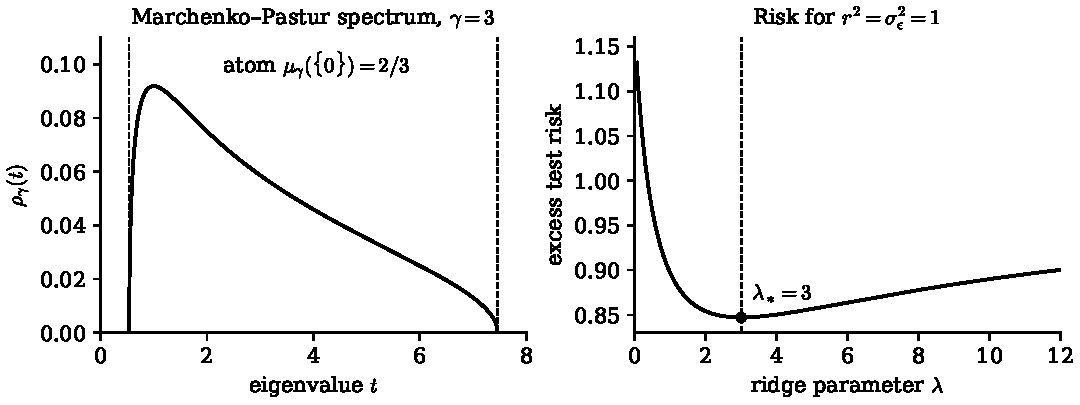
\includegraphics[width=\textwidth]{figures/ridge_gamma3.pdf}
    \caption{
        High-dimensional linear regression at aspect ratio
        \(\gamma=d/n=3\).
        Left: the continuous part of the Marchenko--Pastur spectrum;
        an additional atom of weight \(2/3\) sits at zero.
        Right: the asymptotic excess prediction risk of ridge
        regression for \(r^2=\sigma_\epsilon^2=1\).
        The minimum occurs at
        \(\lambda_*=\gamma\sigma_\epsilon^2/r^2=3\).
    }
    \label{fig:ridge_gamma3}
\end{figure}


% ============================================================
\section{Summary: the recurring idea}
% ============================================================

These examples illustrate the same general principle:
large systems are often controlled not by the raw sizes
individually, but by a small number of \emph{dimensionless ratios}.

\begin{equation}
\boxed{
\begin{array}{ccl}
\text{deep linear network}
&:&
\xi=L/N,
\\[1mm]
\text{ResNet}
&:&
L s_L^2
\quad
\text{(iid case)},
\\[1mm]
\text{high-dimensional regression}
&:&
\gamma=d/n.
\end{array}
}
\end{equation}

The goal of scaling theory is therefore to identify:

\begin{enumerate}
    \item the correct macroscopic variables;
    \item the dimensionless combinations that remain finite;
    \item the corresponding limiting dynamics;
    \item the scaling of hyperparameters required to obtain a
    non-trivial limit.
\end{enumerate}

This is the basic philosophy behind studying neural networks
through large-\(N\), large-\(L\), large-data, and large-training-time
limits.


\end{document}
